%%================================================
%% Filename: chap02.tex
%% Encoding: UTF-8
%% Author: 苏峻锋
%% Created: 2024-02-26
%% Last modified: 2024-02-28
%%================================================
 \chapter{相关理论及技术研究}

\section{服务器集群}

\subsection{服务器集群定义}

服务器集群简称集群(Cluster),由一组线性的服务器组成。
通常将集群中的服务器称作一个节点,集群中各节点之间可以相互通信、协作,
共同组成一个高性能的服务器系统\cite{kanellopoulos2022dynamic}。
来自 Client 的请求由 Cluster 中各服务节点共同处理,同时产生的业务数据通过数据库或者队列等存储形式在各个服务节点之间共享。
从 Client 的角度来看,服务器一整个集群被视作一个整体,服务器集群向客户端忽略了集群中各服务节点之间的通信细节,各服务节点对外实现逻辑同一。

\begin{figure}[ht]
  \centering
  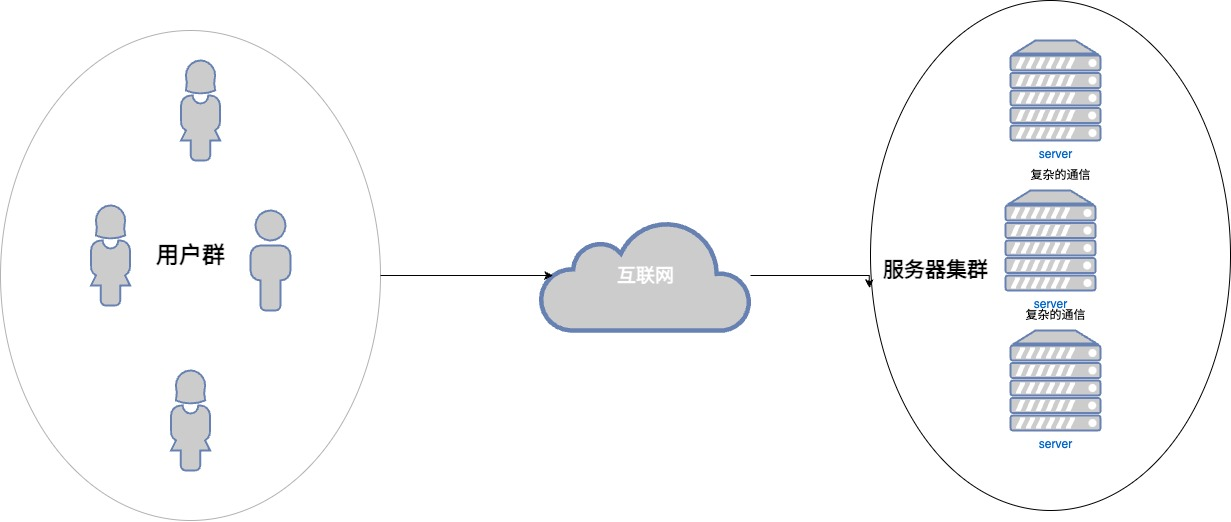
\includegraphics[width=\textwidth]{figures/cluster-and-client.jpg}
  \caption{服务器集群与客户端}
\end{figure}

\subsection{服务器集群的架构优势}

(1)高性能

服务器集群通过协调不同物理硬件性能的服务器,在服务器服务节点处理客户端的请求时,尤其是高并发的场景下,相比于
单个服务器而言,集群架构表现了优越的性能。这种优越的性能不仅仅是不同性能设备能力的叠加,更是因为通信细节的互相协作,紧密联系造就的。

(2)高可用

服务器集群的高可用性体现在服务器集群的容灾和故障转移之上\cite{刘金秀2019基于}。对于大型开发,企业业务来说,服务器的因为处理器负载过高或者其他
导致服务器出现问题而重启崩溃的问题是不可容忍的。集群能够处理这种单独服务器而引发的问题,即使集群中某个服务节点出现故障,
也不能够导致集群不可用,集群中其他服务节点需要立即分摊异常节点的工作。
而只有当集群中所有服务节点同时不可用时,集群才会停止服务。

(3)可伸缩性

可伸缩性实现了对服务器节点灵活管理,并且用户对此并无感知。在负载比较大的情境下,就需要增加对服务器节点的投入,相反
如果负载比较小的情景下,就可以减少集群内的服务器节点

而本文主要优化的方向就是可伸缩性方面,判断不同情境下可能的负载程度,通过对负载情况的预测,能够对实现可伸缩性较大程度的优化。

\subsection{服务器集群的分类}

服务器集群的分类标准有多种,依据不同的标准可以得到不同的集群类别。
例如以多业务结构划分集群,除去常见的同构集群类型外还有目前大量商用化的异构集群。
若以集群实际功能结构划分的话,有三类集群是比较常见的,依次是高性能计算集群、高可用集群以及负载均衡集群\cite{刘卓2017基于Nginx的负载均衡集群设计与实现}。

(1)高性能计算集群

目前高性能计算集一个分支,一直以来都在不断研究多机并行算法及相关软件的开发,
致力于打造超级计算机用于进行复杂的科学运算\cite{xuzongyu}。
通过使用并行计算技术,HPC集群将海量运算问题分解为若干个小部分进行独立运算,
最终结果将由各服务器的计算结果的汇总得到,即通过多台机器提高数据运算的能力,降低数据运算的时间成本。

伴随着当前大数据人工智能技术的发展,HPC集群已经逐渐渗透到科学研究的各个领域,给海量数据运算工作提供了强有力的保障。
高性能计算集群在地形分析、生物制药、数据挖掘以及图像处理等领域发挥着十分重要的作用

(2) 高可用集群

高可用集群顾名思义,即使在高负载、高并发的场景下,可以将该服务器中的服务、资源、IP等转移到另外一台服务器上,从而满足业务的持续性;这两台或多台服务器构成了服务器高可用集群。
简单来说就是京东淘宝24小时不断买买买,微信QQ不断发短信,保证了服务器的不间断运行。然而永远的不间断运行几乎是不可能的,常见的算法并不能彻底处理突然之间的高并发和高负载,比如在双十一期间,某购物网站无法处理突然增加的大量订单
用户刷新造成的DDoS行为,具体衡量标准请看下面这份表。

\noindent\begin{longtblr}[
  caption = {HA衡量标准\cite{信息安全技术信息系统灾难恢复规范}},
  ]{
    hlines,
    vlines,
    % colspec={|X[c]|X[c]|X[c]|X[c]|},
  }
    描述 & 通俗叫法 & 可用性级别 & 年度停机时间 \\
    基本可用性 & 2个9 & 99\% & 87.6小时 \\
    较高可用性 & 3 个9 & 99.9\% 8.8小时 \\
    具有故障自动恢复能力的可用性 & 4 个9 & 99.99\% & 53 分钟\\
    极高可用性 & 5 个9 & 99.999\% & 5 分钟 \\
\end{longtblr}

(3)负载均衡集群

当大量用户并发访问时,将请求转发到不同的机器止实现负载均衡。负载均衡集群是由前端的负载均衡器与后端的服务器构成负载均衡器
介于客户端和服务器之间,通过负载均衡调度策略将负载分发到后端服务器处理,负载均衡集群可以分散单台服务器的访问压力
和存储压力降低单台服务器宕机带来的业务影响\cite{吴宝花2020基于}。为了保证客户端发送的请求能够成功的发送给后端服务器。
处理负载均衡器会判断后端服务器是否正常可用,如果检查到后端服务器状态正常则根据相应的负载均衡策略从这些可用的服务器中选择一台服务器处理对应的请求,
但是如果检查到后端服务器状态异常,则该服务器会被自动剔除待其恢复正常再加入集群系统中。

\begin{figure}[ht]
  \centering
  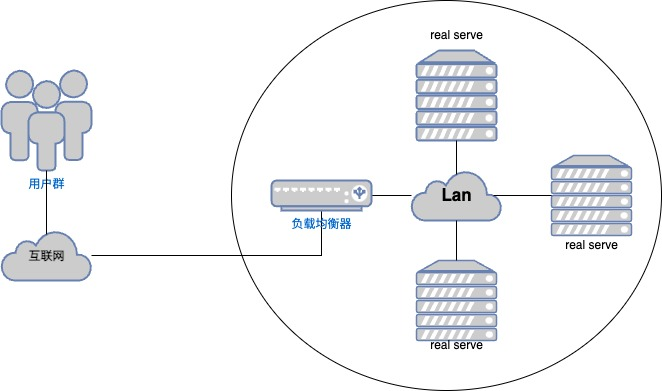
\includegraphics[width=12cm]{figures/负载均衡集群基本结构.jpg}
  \caption{负载均衡集群的基本架构}
\end{figure}

但是负载均衡集群存在一定的缺陷,负载均衡器无法对集群服务器性能进行监控,因而分配请求时容易导致服务器过载或者空闲情况的出现。
针对这种情况,该类集群将收集业务服务器动态负载状况的性能监控程序部署在请求分发服务器上,通过对该程序的使用可以时时刻刻掌握
上游服务器的负载变化。本论文的研究内容即是负载均衡集群下深度学习算法的使用。

\subsection{服务器性能指标}

负载均衡集群通过使用性能监控程序观察上游服务器的性能情况,要达到这一点,其中最主要的一点是如何选取评价节点当前负载状况的指标,且这些指标获取简单,获取时占用
系统资源少,更能有效的反映出的服务器节点的资源使用情况,可以将这些指标称作为负载向量。通过研究发现,反应服务器性能指标通常从这几个方面考虑:
CPU,内存,网络带宽,磁盘I/O,通过研究发现,采用不同的性能评价指标对负载均衡算法有较大的改变,而随着应用环境的改变,评价指标也会有不同的变化。

通过监控资源利用率(如 CPU、内存、磁盘 I/O 和网络带宽),系统可以确保工作负载均匀分布在所有可用资源上。
这样可以确保没有任何单个资源的过度使用,从而最大化整体性能。当业务增长时,可以根据资源利用率数据来决定何时需要
扩展硬件或调整系统配置,以优化性能和成本。

计算机一个重要的硬件就是 CPU,通常CPU的利用效率就几乎相当于服务器节点的性能情况,如果利用率过高,那么性能就会变低,
负载程度变大。每个 CPU 的大小核和频率也是影响 CPU 性能的重要组成条件,每个CPU的型号不同,那么需要将CPU性能作为负载向量的评价也就越难。
服务器节点的内存访问速率对 CPU 的任务处理效率影响较大。
而当网络请求量的增加带来的数据访问也会不断增加,在内存中数据请求和移动造成的分页错误或缺页的概率也会不断上升。
这样会严重影响CPU中任务处理效率,服务器节点处理请求任务的效率下降,导致集群整体的性能下降

如果主要对服务器的计算有着高性能的需求,那么最好将 CPU 和内存作为重要的评价指标,
若是处理的任务需要频繁的进行数据的传输和存储,那么网络和磁盘 I/O 对这种任务类型的影响更大。

上述负载向量指标只是服务器节点实时的工作状态\cite{mahato2017scheduling},而队列的长度是节点处理请求任务的,完成某项任务的整个流程法人方向来思考的,这种方式具有预测性的。
此时,如果有任务入队列,那么此时的服务器节点负载程度比较高,并不能接受更多的任务。性能监控程序只能监控当先服务器的实时性能,但是网络任务是作为队列被负载均衡器分发的
虽然能够判断队列的长度,但是队列里对任务消耗资源的能力是无法得知的,所以任务队列的长度不能准确反应节点的负载能力。队列一般考虑的是 CPU 的队列长度
获取 CPU 的队列长度,可以通过两个视角来呈现,其一是获取 CPU 一段时间内的平均队列长度,其二是获取 CPU 某个时刻的队列长度。

由于不能简单的使用 CPU 性能和任务队列长度作为负载向量指标,所以我们需要一个综合的负载信息评价标准,获取多种不同的指标信息,
经过数学运算,得到一个能够从多方面体现节点负载程度的新指标。通过对黄伟华,一种特征加权模糊聚类的负载均衡算法\cite{黄伟华2017一种特征加权模糊聚类的负载均衡算法}
 的研究,主要有三种方法。第一种方法既是使用队列长度作为主要指标,同时考虑使用 CPU 和磁盘IO 作为次要指标;另一种是完全结合,同时将队列的长度和资源利用
率作为参考指标;最后一种是通过优先级作为主要指标,比如内存占用情况,在内存充足的情况下,在考虑其他次要的指标。

\subsection{本文选择的参考指标}

依据自身经济和技术情况,选择使用观察节点的各种资源利用情况作为负载均衡能力的指标,并选取了 CPU,内存,磁盘 I/O 和网络带宽作为评价各个节点性能的指标。
具体的系统状态评价对应的资源利用率情况本文进行了整理,如下图表所示。

\noindent\begin{longtblr}[caption={稳定系统的资源状态和评价}]
  {hlines,vlines, colspec = {X[c]X[c]X[c]}}
  性能指标 & 资源利用率 & 状态评价 \\ 
  \SetCell[r=3]{c} CPU 利用率 & 70\% & 好 \\
                              & 85\% & 坏 \\
                              & 90\%+ & 很差 \\
  \SetCell[r=3]{c} 磁盘IO & <30\% & 好 \\
                          & <40\% & 坏 \\
                          & <50\% & 很差 \\
  运行队列 & <2*CPU数量 & 好 \\
  网络带宽 & <30\%带宽 & 好 \\
  \SetCell[r=3]{c} 内存 & 没有页交换 & 好 \\
                        & 每个 CPU每秒10个页交换 & 坏 \\
                        & 更多的页交换 & 很差\\
\end{longtblr}

设 $C_j$、$M_j$、$D_j$、$M_j$ 分别作为第 j 个节点的 CPU 剩余性能,内存剩余性能,磁盘剩余性能,网络带宽剩余性能。
在服务器集群处理大量任务和网络请求时,由于分发的请求量和请求所处理的数据量的不同,可能会出现有的节点处于高负载,
有的节点处于低负载的情况,这样服务器集群的性能就不能得到充分的发挥,所以需要一直监控集群中
各个节点的负载状况,不断调整任务队列的分配方案。下面是计算当前服务器节点的负载状态的数学公式
\[
  U_j = 1000 \cdot (W_{cpu} \cdot C_j + W_{mem} \cdot M_j + W_{io} \cdot D_j + W_{net} \cdot N_j)\tag{1.1}
\]
$U_j$ 为当前服务器节点的总体剩余性能。通过对 $U_j$ 值的监控,观察其变化范围作为判断是否需要修改请求人文分配方案的依据。

\section{负载均衡技术}

\subsection{什么是负载均衡}

负载均衡是在支持应用程序的资源池中平均分配网络流量的一种方法。现代应用程序必须同时处理数百万用户,并以快速、可靠的方式将正确的文本、视频、图像和其他数据返回给每个用户。为了处理如此高的流量,大多数应用程序都有许多资源服务器,它们之间包含很多重复数据。负载均衡器是位于用户与服务器组之间的设备,充当不可见的协调者,确保均等使用所有资源服务器。

\subsection{负载均衡的优势}

负载均衡可以定向和控制应用程序服务器与其访客或客户端之间的互联网流量。因此,它可提高应用程序的可用性、可扩展性、安全性和性能。

(1)应用程序可用性

服务器故障或维护可能会增加应用程序停机时间,使访客无法访问应用程序。
负载均衡器可以通过以下方式提高系统的容错能力,自动检测服务器问题并将客户端流量重定向到可用服务器。
运行应用程序服务器维护或升级而无需使应用程序停机,为备份站点提供自动灾难恢复,
执行运行状况检查并防止出现可能导致停机的问题。

(2)应用程序可扩展性

可以使用负载均衡器在多个服务器之间智能地定向网络流量。
应用程序可以处理数千个客户端请求,防止任何一台服务器出现流量瓶颈,
预测应用程序流量,以便可以在需要时添加或移除不同服务器,
为系统增加冗余度,使我们可以放心扩展。

(3)应用程序安全

负载均衡器具有多项内置的安全功能,它们是应对分布式拒绝服务攻击的有用工具,
在这种攻击中,攻击者会用数百万个并发请求淹没应用程序服务器,从而导致服务器故障。负载均衡能够做到:
监控流量并阻止恶意内容,预测应用程序流量,
将攻击流量自动重定向到多个后端服务器,以最大限度减少影响,
通过一组网络防火墙路由流量,以提高安全性。

(4)应用程序性能

负载均衡器通过增加响应时间和减少网络延迟来提高应用程序性能。它们可以执行诸如以下几项关键任务:
在服务器之间平均分配负载以提高应用程序性能,将客户端请求重定向到地理位置较近的服务器以减少延迟;
确保物理和虚拟计算资源的可靠性和性能。

\subsection{负载均衡的类型}

实现负载均衡的方式有很多种,最常见的时间负载均衡类型有三种。

(1)软件和硬件负载均衡

基于硬件的负载均衡器是一种硬件设备,可以安全地处理千兆字节的流量并将其重定向到数百个不同的服务器。可以将其存储在数据中心,并使用虚拟化创建多个可以集中管理的数字或虚拟负载均衡器。
基于软件的负载均衡器是执行所有负载均衡功能的应用程序。可以将它们安装在任何服务器上,也可作为完全托管的第三方服务的形式访问。

硬件负载均衡器需要初始投资、配置和持续维护。也可能不会满负荷使用它们,尤其只是为了处理高峰时段的流量高峰。如果流量突然增加到超出其当前容量,这将影响用户,
直到能购买并设置另一个负载均衡器为止。
相比之下,基于软件的负载均衡器要灵活得多\cite{常智2013高性能}。
它们可以轻松地纵向扩展或缩减,并且与现代云计算环境更加兼容。随着时间推移,它们的设置、管理和使用成本也会降低。

(2)静态和动态负载均衡

静态负载均衡是根据相关规则制定的负载均衡算法,典型的静态负载均衡策略有加权轮询、IP-HASH等。
静态负载均衡又称作确定性调度,这是由于在请求分发过程中该类策略不会考虑服务器实际运行时的负载性能,
这就容易导致出现性能好的服务器处于过载而性能一般的服务器处于轻载甚至空闲状态的不均衡状况,
集群资源利用率得不到充分发挥,系统性能被大大削减。静态负载均衡容易实现,配置简单,
因此也是比较常见且应用较多的一种负载均衡实现方式。

动态负载均衡的实现需要更为复杂的技术支撑,它在静态负载均衡的实现基础上,
需要对集群系统各服务器的运行状态加以评估,通过某些反映服务器运行时负载情况的负载评价指标的变化来动态调节各服务节点的请求分发比例,
从而能够将集群系统的资源充分利用在处理高并发客户端请求上,以达到集群负载动态均衡的目标。
在实践中,动态负载均衡能够大大提升集群系统的负载性能,但其实现是建立在一定量的系统资源消耗之上,对于一些没有资源的企业来说可能有点困难,但是对于大型企业来说这些成本就可以忽略不计。

根据负载均衡技术类型的不同,下表分析了常见的 Nginx 负载均衡策略。

\noindent\begin{longtblr}
  [caption = {常见 Nginx 负载均衡算法分析表}]
  {
    hlines,
    vlines,
    colspec = {X[c]X[c]X[l]X[l]},
  }
  负载均衡算法分类 & 算法名 & 优点 & 缺点 \\
  \SetCell[r=3]{c} 静态负载均衡 & 轮询算法 & 配置简单 & 不能考虑后端服务器性能差异 \\
                                & 加权轮询算法 & 能够考虑不同服务器的性能差异 & 不能考虑负载后服务器的状态变化 \\
                                & IP 哈希法 & 可以解决 session 问题 & 但在 Nginx 非最前服务器后失效 \\
  \SetCell[r=4]{c} 动态负载均衡 & 平均分配认为 & 不能考虑服务器处理能力不同 \\
                                & 加权最小连接法 & 考虑处理能力的不同 & 无法衡量服务器负载状态 \\
                                & 最短响应时间法 & 根据服务器响应时间分配请求 & 通信开销过大 \\
                                & 基于资源的方法 & 性能最大化,控制分散灵活 & 配置复杂,不一定反映实际负载 \\
\end{longtblr}

(3)四层到七层负载均衡

大型的网站服务一般会用这样的架构,在业务应用前面加七层负载均衡,然后在七层负载均衡前面加四层负载均衡。当用户发送 HTTP 请求的时候,请求会(经过机房内的路由器,交换机等设备)首先到达四层负载均衡,四层转发给七层,七层转发给应用。
四层负载均衡只解析网络包到第四层,根据四层的内容(比如 TCP port,IP 等)就能确定转发给谁,
七层负载均衡解析网络包到第七层,要根据七层的内容(比如 HTTP URL path,HTTP header 等)才能确定转发给谁。

七层即应用层\cite{pak2015efficient},要解析 HTTP 内容(不仅仅是 HTTP,其他应用层协议的负载均衡,比如一些数据库 proxy,gRPC 代理,等等,
都需要解析完成应用层才能确定转发目标),首先要将 Header 全部读完,读完之后要看下
Content Length 是有多长,然后知道 Body 要读到哪里。根据不同的 URL Path,
还要确定路由到哪一个 upstream。


四层即传输层,对于用户任务,四层负载均衡器首先通过预先配置好的负载均衡策略在内部网络
中挑选一台最好的服务器,接着将请求报文中的目标IP地址和端口号修改为内部最佳的服务器IP和端口号
并建立TCP链接转发请求,最后将响应结果返回给用户。用 Nginx 模拟四层负载均衡如下图所示。

\begin{figure}[htb]
  \centering
  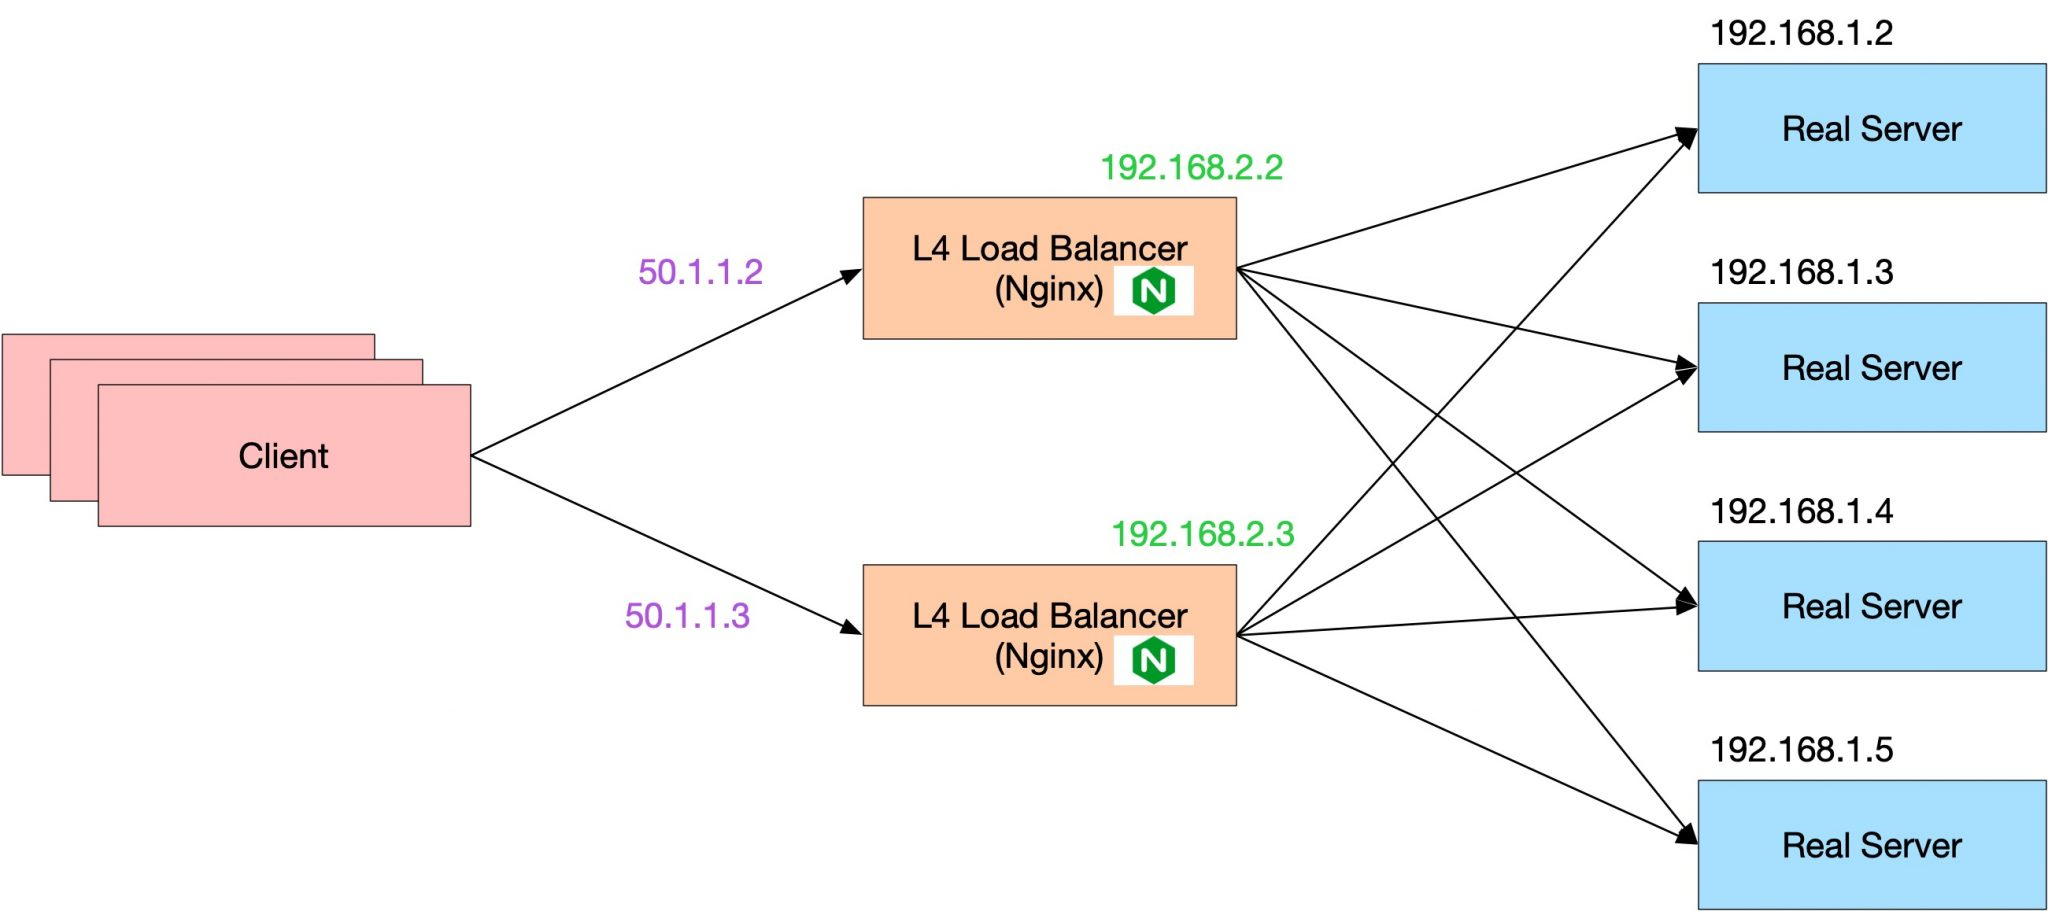
\includegraphics[width=\textwidth]{figures/nginx-l4lb-2048x911.jpg}
  \caption{Nginx 作为四层负载均衡使用}
\end{figure}

\newpage

\section{Nginx 服务器}

Nginx是一款轻量级的Web服务器/反向代理服务器及电子邮件代理服务器。本身具有占用内存少,并发能力强等特点,其并发能力在同类型的网页服务器中表现较好。
Nginx是由伊戈尔·赛索耶夫为俄罗斯访问量第二的Rambler.ru站点开发的,第一个公开版本0.1.0发布于2004年10月4日。
Nginx 相较于之前盛行的 LAMP(Linux Apache MySQL PHP/Python/Perl)由于 Apache 服务器同步多进程的处理方式,
而 Nginx 是基于事件驱动架构,在处理任务请求是异步而非阻塞的,因此应对高并发请求是以就能够保持资源的低消耗、响应能力迅速以及稳定性强的特点\cite{凌质亿2013高并发环境下}。包括百度,京东等众多服务器都是采用Nginx。

\subsection{Nginx 工作模式和进程模型}

Nginx 有单进程和多进程两种工作模式,默认进程为多进程。通常情况下,单进程仅仅只在开发环境下调试使用,对外发布服务时
常常使用多进程。多进程模型既是 master-worker 进程模型

\noindent\begin{enumerate}
  \item Nginx 启动后,会产生一个 master 主进程,主进程执行一系列的工作后会产生一个或者多个工作进程 worker
  \item 在客户端请求动态站点的过程中,Nginx 服务器还涉及和后端服务器的通信。Nginx 将接收到的 Web 请求通过代理转发到后端服务器,由后端服务器进行数据处理和组织
  \item Nginx 为了提高对请求的响应效率,降低网络压力,采用了缓存机制,将历史应答数据缓存到本地。保障对缓存文件的快速访问
\end{enumerate}

首先,worker 进程之间是平等的,每个 worker 进程都是从 master 进程 fork 过来,
在 master 进程里面,先建立好需要 listen 的 socket(listenfd)之后,
然后再 fork 出多个 worker 进程。每个 worker 进程,处理请求的机会也是一样的。
所有 worker 进程的 listenfd 会在新连接到来时变得可读,为保证只有一个进程处理该连接,
所有 worker 进程在注册 listenfd 读事件前抢 accept\_mutex,抢到互斥锁
的那个 worker 进程注册 listenfd 读事件,在读事件里调用 accept 接受该连接。
当一个 worker 进程在 accept 这个连接之后,就开始读取请求,解析请求,处理请求,产生数据后,
再返回给客户端,最后断开连接,这样就是一个完整的请求就是这样的了。

具体图示如下

\noindent\begin{figure}[htb]
  \centering
  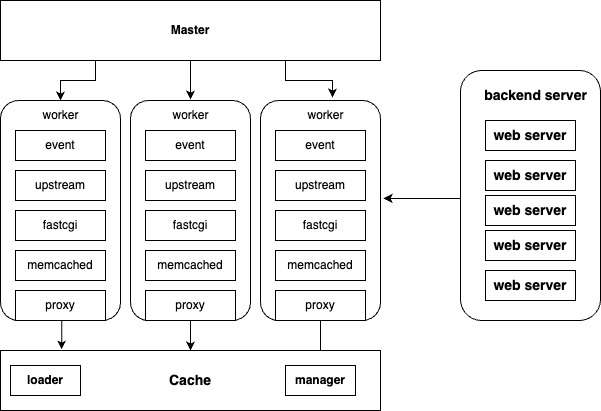
\includegraphics[width=0.8\textwidth]{figures/master-worker.jpg}
  \caption{Nginx 多进程工作模式}
\end{figure}

由于 Nginx 底层基于 epoil 事件驱动模型实现异步非阻塞 IO,一个进程可以监听多个 socket,因此每一个 worker 进程
都可以并发多个链接甚至上万个连接\cite{张炜森2018nginx},这保证了 Nginx 的高并发性能,而且消耗的内存非常少。

\subsection{Nginx的反向代理}

代理简单来说,就是如果我们想做什么,但又不想直接去做,那么这时候就找另外一个人帮我们去做。那么这个例子里面的中介公司就是给我们做代理服务的,我们委托中介公司帮我们找房子。
弄清楚代理是什么了,既然有反向代理,那么正向代理是什么?先从反向代理解释起。
反向代理,其实客户端是没有任何感知的,因为客户端不需要任何配置既可以访问。
我们只需要将请求发送到反向代理服务器,由反向代理服务器去选择目标服务器获取数据后,在返回给客户端,此时反向代理服务器和目标服务器对外就是一个服务器,暴露的是代理服务器地址,隐藏了真实服务器IP地址。

理解这两种代理的关键在于代理服务器所代理的对象是什么,正向代理代理的是客户端,我们需要在客户端进行一些代理的设置。而反向代理代理的是服务器,作为客户端的我们是无法感知到服务器的真实存在的。
总结起来就一句话:正向代理代理客户端,反向代理代理服务器\cite{崔娟2023基于Nginx反向代理解决公网上服务跨域问题的研究}。

用一个图片对比正向和反向代理

\begin{figure}[htb]
  \centering
  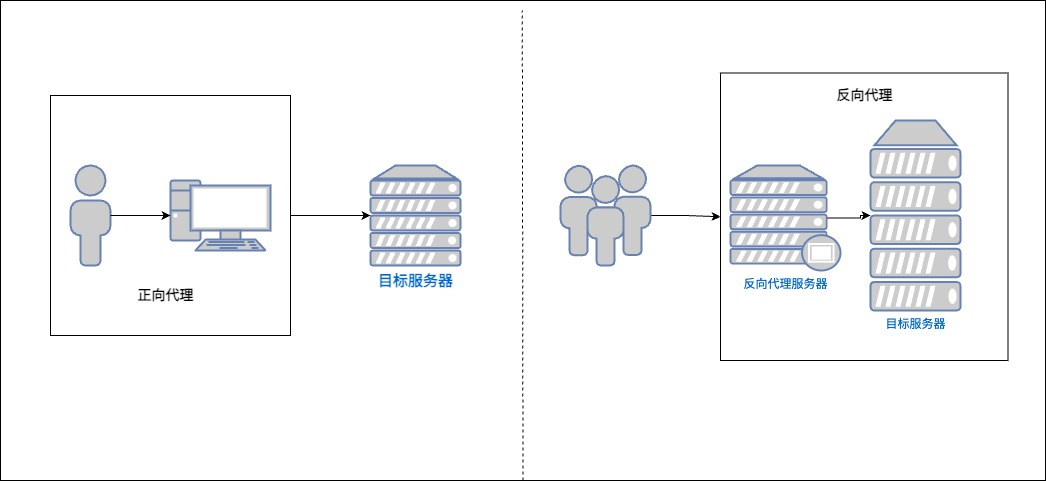
\includegraphics[width=\textwidth]{figures/Forward-Proxy-Reverse-Proxy.jpg}
  \caption{正向代理与反向代理的对比}
\end{figure}

Nginx反向代理功能使其能够逾越单机的局限性,并拥有在网络上接收、转发以及处理数据的能力\cite{马原龙2016nginx}。
通过proxy\_pass指令可以配置Nginx反向代理,proxy\_pass的语法结构为proxy\_passURL,
这个URL即表示Nginx所代理的上游服务器地址信息。
Nginx反向代理的一个配置实例如下所示,配置中的“proxy\_set\_headerX-Real-IP”表示定义了一个值为“\$remote\_addr”的首部“X-Real-IP”,
也即客户端的IP地址。当上游服务器接收到客户端请求时,该自定义的首部将以客户端IP的形式被打印到服务器访问日志中,
上游服务器便能够依据真实客户端的IP地址而非Nginx的IP地址做日志统计分析\cite{吴陈2020基于Nginx的服务器集群负载均衡策略的研究与改进}。

\newpage

\noindent \begin{lstlisting}[caption={Nginx 反向代理默认配置}]
location \index{
  set $upstream_url "";
  proxy_set_header X-Real-IP $remote_addr;
  rewrite_by_lua_file /home/${HOME}/luafile/log.lua
  proxy_pass http://upstream_url;
}
\end{lstlisting}

在客户端与 Nginx 通信过程中,当请求到达 Nginx 服务器时,Nginx 并不能立即与目标服务器建立 TCP 连接
而转发请求工作,而是将任务请求储存在内部缓存队列中,之后在与目标服务器通信发送请求,这种工作模式大大降低里服务器某一节点的负载压力。
另外,由于客户端与 Nginx 是在公网上进行网络通信传输,属于慢速连接,而 Nginx 与上游服务器一般是在内部网络进行通信,属于高速连接,考虑到 HTTP 连接具有无状
态性,客户端与 Nginx 可以开启 Keep-Alive 功能,Nginx 与上游服务器之间的 Keep-Alive
则可以关闭,因此更能将占用上游服务器的系统资源释放掉,进一步减轻服务器负载。

当上游服务器针对客户端HTTP请求处理结束并生成响应报文发送给Nginx反向代理服务器后,
Nginx首先将拆开报文进行相关处理,二次封装完成响应给客户端。
在这个过程中,Nginx是在接收上游服务器传来的响应报文的同时向客户端发送响应报文,
而不像客户端请求资源时Nginx先接收,接收完成后再发送给上游服务器的情况一样,
Nginx边接收边转发的工作模式可以极大地减小客户端响应的延迟\cite{邓仲举2012高可靠性集群部署的设计与实现}。

\subsection{Nginx 负载均衡}

Nginx 自身支持多种负载均衡算法,除了使用源码自带的内置调度算法之外,还可以支持第三方扩展的
负载均衡技术\cite{sufiev2016dynamic}。如果想要开启源码自带的调度算法可以则可以把指定调度算法
的模块打开。一般来说,不需要单独下载某一模块,需要使用时在配置文件中指定即可。Nginx 内置的调度
算法有加权轮询算法、最小连接算法、IP 哈希算法。第三方扩展算法则需要安装第三方模块,将模块放在指定的扩展算法
模块路径,在编译Nginx过程中,扩展算法会一并编译在二进制程序中,最后使用便可以依据配置指令使用指定的
第三方调度算法。常见的第三方调度算法有 fair 响应时间比算法(需要安装ngx\_http\_upstream\_fair\_module),URL 哈希算法(需要安装ngx\_http\_upstream\_hash\_module)
等。下面将对常见的Nginx调度算法进行分析。

(1)加权轮询算法

默认轮询算法(Round Robin)的策略是:将请求“依次”分发到候选机器。如下图所示,轮询负载均衡器收到来自客户端的 6 个请求,编号为 1、4 的请求会被发送到服务端 0;编号为 2、5 的请求会被发送到服务端 1;编号为 3、6 的请求会被发送到服务端 2。

\begin{figure}[htb]
  \centering
  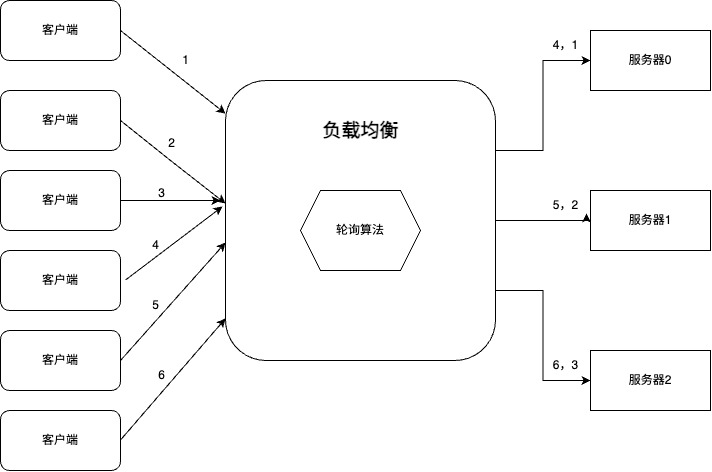
\includegraphics[width=\textwidth]{figures/round-robin.jpg}
  \caption{默认情况下的负载均衡算法}
\end{figure}

默认的轮询算法是等值轮询,即按照一比一的比例向不同的服务器节点分发请求,当配置文件
没有任何 weight 权值参数是,则采用默认的轮询算法。于是加权轮询算法则考虑了不同性能特点
的服务器节点,性能好的服务器则设置较大的权值,性能不好的服务器则设置较小的权值。
当任务入队列时负载均衡器则可以按照设置好的权值比例合理的悬着服务器执行请求调度

\begin{lstlisting}
# 默认的轮询算法
upstream backend {
    server 127.0.0.14:80 max_fails=2 fail_timeout=10s;
    server 127.0.0.15:80 max_fails=2 fail_timeout=10s;
}
# 加权轮询算法
upstream backend {
    server 127.0.0.14:80 weight=5 max_fails=2 fail_timeout=10s;
    server 127.0.0.15:80 weight=10 max_fails=2 fail_timeout=10s;
}
\end{lstlisting}

通过对 Nginx 源码的研究,在 ngx\_http\_upstream\_round\_round\_robin.c 这个文件下 ngx\_http\_upstream\_get\_round\_robin\_peer
函数是对加权轮询算法的实现。在具体分配任务的环节,为了记录上游集群节点服务器的权值公设有四个变量,
依次是 weight、effective\_weight、total 和 current\_weight。

\noindent\begin{longtblr}
  [caption = {加权轮询算法变量及描述}]
  {hlines, colspec = {|X[1, c]|X[2, c]|}}
  变量 & 描述 \\
  weight & 初始权值,固定不变 \\
  effective\_weight & 发生错误,权值减小 \\
  total & 集群服务器权值总和 \\
  current\_weight & 实时权值,初始为零 \\
\end{longtblr}

在一次任务中,负载均衡器勉励上游服务器节点的 current\_weight 加上起对应的有效权值 effective\_weight,
负载均衡器将会选择 current\_weight 最大的服务器节点为本轮最佳服务器。当该服务器正在进行任务时,负载均衡器会
降低其 current\_weight。Nginx 定义了两个事件状态,NGX\_OK 表示成功选择最佳服务器,NGX\_BUSY 表示服务器选择失败
或者通信发生错误。加权轮询算法详细流程如下图2.8 所示。

\begin{figure}[htb]
  \centering
  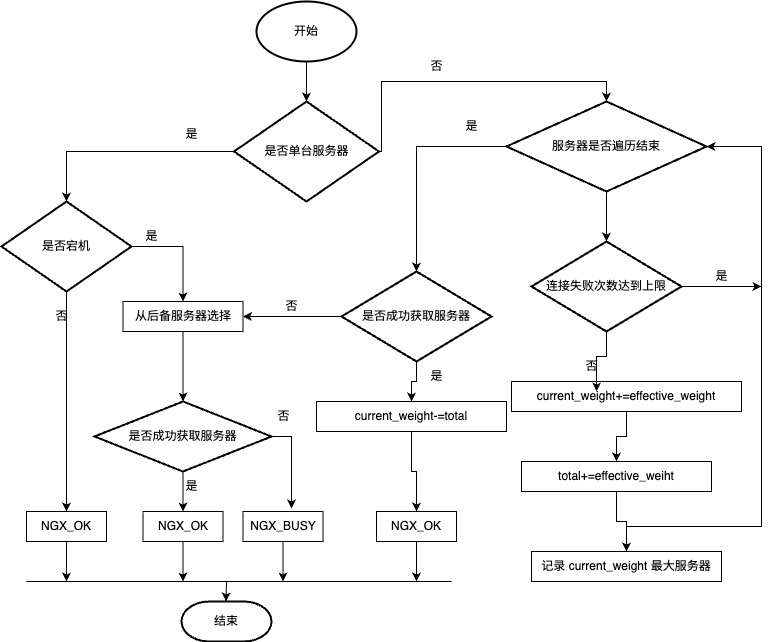
\includegraphics[width=\textwidth]{figures/round-flowchart.jpg}
  \caption{Nginx 加权轮询算法流程图}
\end{figure}

加权轮询算法,虽然考虑了上游服务器节点的不同性能差异,算法的复杂度比较低,执行效率较高,节点选择频次相对平滑,
配置简单,但是在具体任务过程中,有些任务比较繁忙,有些任务比较轻松,这种静态的权重调节无法根据真实负载
情况进行动态调整。为了解决这个问题,诞生了动态权值的加权轮询算法,基于手机各个后台服务器节点工作时的 CPU
利用率、内存利用率、网络性能和磁盘IO等性能情况,动态的调整后端服务器节点权重\cite{谭畅2021云中心基于}。该算法在高并发
的场景下,响应时间和实际并发方面表现更好。

(2)最小连接算法

最小连接算法(least\_conn)一句话概括就是:按nginx反向代理与后端服务器之间的连接数,连接数最少的优先分配\cite{周常志2023基于改进加权最小连接数的微服务负载均衡算法研究}。
要根据机器连接数分发,显然要先维护机器的连接数。
因此,最少连接数算法需要实时追踪每个候选机器的活跃连接数;
然后,动态选出连接数最少的机器,优先分发请求。最少连接数算法会记录当前时刻,
每个候选节点正在处理的连接数,然后选择连接数最小的节点。该策略能够动态、
实时地反应机器的当前状况,较为合理地将负责分配均匀,适用于对当前系统负载较为敏感的场景。

\begin{lstlisting}
# 最小连接算法
upstream backend {
    least_conn;
    server 127.0.0.14:80 max_fails=2 fail_timeout=10s;
    server 127.0.0.15:80 max_fails=2 fail_timeout=10s;
}
\end{lstlisting}

最小连接数调度算法每一个上游集群节点分别维护一个计数变量 number,每次负载均衡器分配个某一节点一个
任务时,就将其对应的 number 值上加上 1,当任务完成之后,再将 number 值减去 1。Nginx 根据集群各服务器
计数变量的变化,每次都会挑选 number 数值最小的服务器进行任务分配。同时最小连接算法与加权连接算法接轨,
如果初始为每一个性能各异的服务器分配初始权重,那么当分发任务请求时将选择连接数与权值比例最小的服务器
节点作为最佳服务器节点。最小连接算法流程图如下如下图所示。

\begin{figure}[htb]
  \centering
  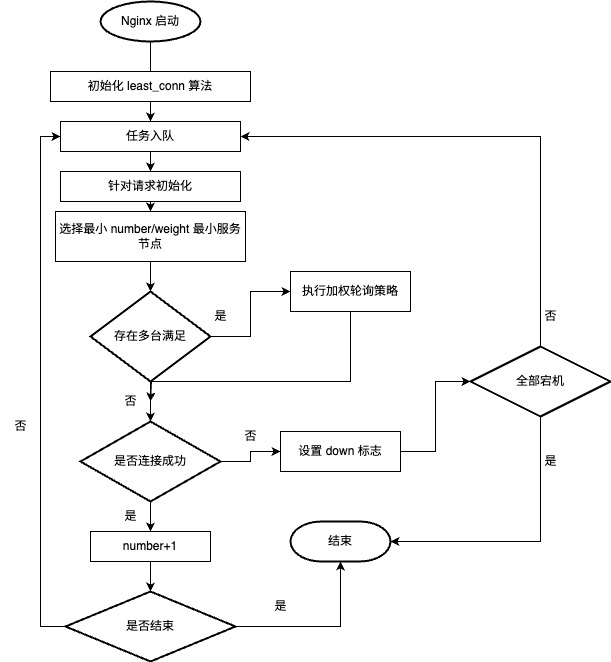
\includegraphics[width=\textwidth]{figures/least-flowchart.jpg}
  \caption{Nginx 最小连接算法}
\end{figure}

最小连接算法根据服务器连接数大小变化的统计结果来动态的选择服务器分发任务,对于服务器的实时
负载情况做了些许的考虑,一定程度上解决了加权轮询算法中请求到来时间间隔不一致所带来的负载差异。
但由于每条连接上的请求不同,该算法但从连接数大小来反应实时负载情况还是不够全面。

(3)IP 哈希算法

哈希算法(Hash)根据一个 key (可以是唯一 ID、IP、URL 等),通过哈希函数计算得到一个数值,用该数值在候选机器列表的进行取模运算,得到的结果便是选中的机器\cite{邱亚飞2021哈希算法的实现与验证}。
哈希算法解决的问题既是人工的判断某个具体任务需要的性能大小,如果该任务消耗的性能较多,负载均衡器将会对该请求连接进行分配到候选的高性能服务器中。
这种算法可以保证,同一关键字(IP 或 URL 等)的请求,始终会被转发到同一台机器上。哈希负载均衡算法常被用于实现会话粘滞(Sticky Session)。
但是 ,哈希算法的问题是:当增减节点时,由于哈希取模函数的基数发生变化,
会影响大部分的映射关系,从而导致之前的数据不可访问。要解决这个问题,
就必须根据新的计算公式迁移数据。显然,如果数据量很大的情况下,迁移成本很高;
并且,在迁移过程中,要保证业务平滑过渡,需要使用数据双写等较为复杂的技术手段。

\begin{figure}[htb]
  \centering
  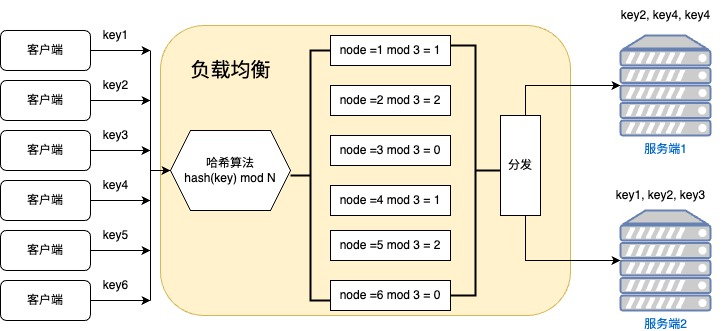
\includegraphics[width=\textwidth]{figures/hash-algo.jpg}
  \caption{Nginx 哈希算法拓扑图}
\end{figure}

Nginx 的IP 哈希算法则是将来源客户端的IP地址作为key,采用特定的哈希函数作哈希运算,最后将结果请求转发到特定的服务器上进行处理。
Nginx 负载均衡器受到客户端请求后,将该客户端的点分十进制前三段作为参数输入到哈希函数计算,哈希值的以保证 IP 地址前三段能够分发导通一个上游服务器,哈希
计算完成之后将此 hash 值 对集群中所有正常运行的服务器总数进行趋于,用来确定将任务请求分发到那台服务器上。在确定服务器节点过程中,
如果失败次数超过 20 次,将会替换为加权轮询策略。Nginx 配置 IP 哈希算法如下所示。

\begin{lstlisting}
# IP-HASH 算法
upstream backend {
    ip_hash;
    server 127.0.0.14:80 max_fails=2 fail_timeout=10s;
    server 127.0.0.15:80 max_fails=2 fail_timeout=10s;
}
\end{lstlisting}

IP 哈希算法流程图如下所示。

\begin{figure}[htb]
  \centering
  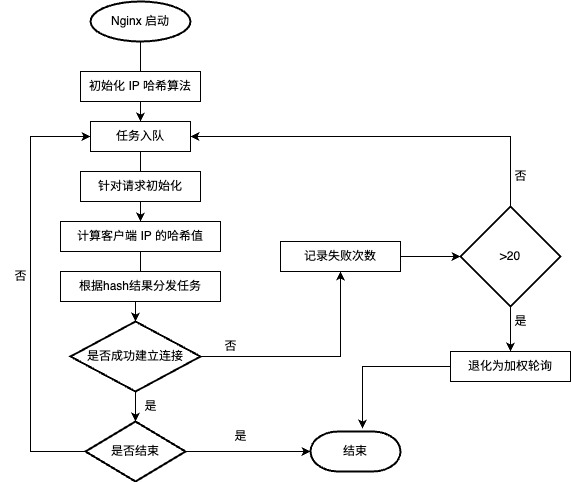
\includegraphics[width=\textwidth]{hash-flowchart.jpg}
  \caption{Nginx IP 哈希算法流程图}
\end{figure}

IP 哈希算法能满足用户会话保持的要求,因为同一个IP的用户请求将映射导通一个服务器节点进行处理。
当集群节点出现故障或者集群加入新节点,需要重新进行哈希运算,因此仍旧会出现会话沾性失效问题。
在资源占用率比较高的高并发情景下,IP 哈希算法对于不同资源的消耗仍旧无法考虑,还是容易导致某一个服务器节点过载而崩溃
而其他节点过于空闲的状态。所以任何不能彻底的明白每一个集群节点中的实时负载的负载均衡算法都无法保证节点是否过载或者过于空闲。

在上述的 Nginx 几种内置的常见调度算法,常见的扩展调度算法还有最小响应比算法。
fair 算法在分配客户端请求时依据上游服务器的响应时间作为参考量,将处理请求的高优先级赋予响应时间短的服务器,
由于响应时间越长的服务器负载相对越重,因此优先级滞后。fair 算法依据页面大小和加载时间长短能够自适应地进行负载均衡,
在一定程度上考虑到了上游服务器的性能差异。但在高并发情况下,没有考虑到网络拥塞可能带来的耗时延长的情况,
且单靠响应时间来判断负载过于片面,不够准确可靠\cite{张艳肖2023基于Fair函数神经网络的厚度传感器输出特性分析}。

经过上面的对Nginx几种内置的负载均衡算法可以得知,静态负载均衡算法配置一遍比较简单,而且执行效率很好,一定程度上能够反应集群节点的负载性能。
而动态负载均衡则配置比较复杂,在不考虑多方面的情况下,不够准确可靠,但是相比于静态负载均衡能够更加实时的了解某一节点的性能状态,以至于能够让
负载均衡器更好的分配工作。于是本文将从机器学习和神经网络方面探究动态负载均衡中关于网络方面的优化,并分析结果加以与原来对比。

\section{本章小结}

本章主要阐述了常规负载均衡算法探究涉及的相关理论和技术。首先介绍了服务器集群的概念和分类,
同时确定了如何测量服务器剩余节点性能的标准。其次分析了负载均衡技术的意义与优势,在分析负载均衡类型的过程中
确认了要突破的方向。最后通过对于Nginx 源码的了解探究了 Nginx 的工作模式和进程模型,了解了常规的负载均衡算法以及实现,
让我明确了向动态负载均衡算法中关于网络方面的研究方向。
